\usetikzlibrary{decorations.pathmorphing}
\usetikzlibrary{decorations.markings}
\usetikzlibrary{decorations.pathmorphing}
\usetikzlibrary{arrows}
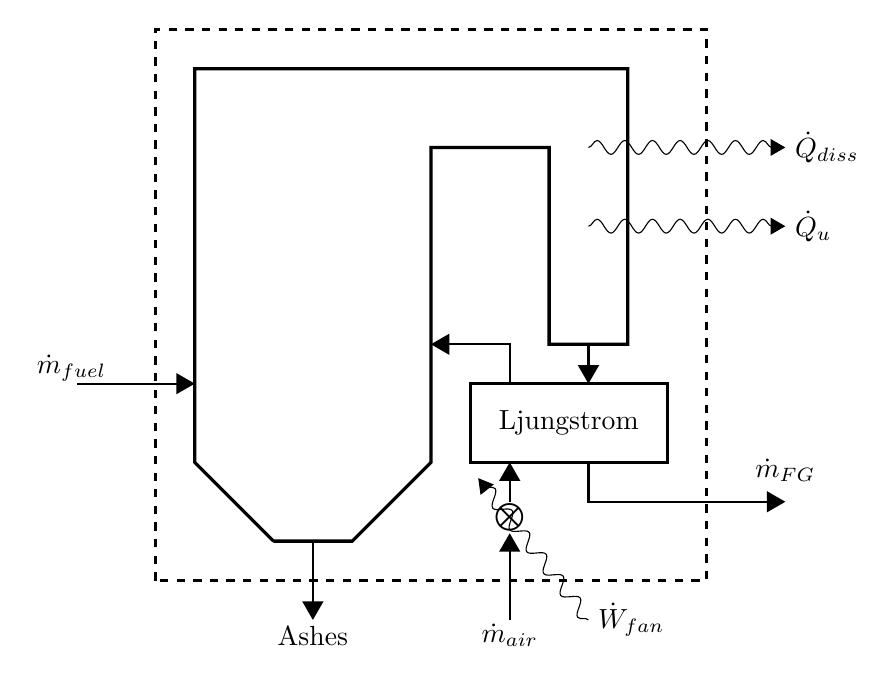
\begin{tikzpicture}[>=triangle 60]
% rectangle
\draw[dashed,very thick] (-0.5,-0.5) rectangle (6.5,6.5);
%main
\draw[very thick] (1,0)--(0,1)--(0,6)--(5.5,6)--(5.5,2.5)--(4.5,2.5)--(4.5,5)--(3,5)--(3,1)--(2,0)--(1,0);
% ljungstrom
\draw[very thick] (3.5,1) rectangle (6,2);
\node[] at (4.75,1.5) {Ljungstrom};
% flue gas
\draw[thick,->]  (5,2.5)--(5,2);
\draw[thick,->]  (5,1)--(5,0.5)--(7.5,0.5);
\node[] at (7.5,0.9) {$\dot{m}_{FG}$};
% fan
\node[very thick] at (4,0.3) {$\bigotimes$};
%\draw[very thick] (4,0.3) circle (0.3);
% air before fan
\draw[thick,->]  (4,-1)--(4,0.1);
\draw[thick,->]  (4,0.5)--(4,1);
\node[] at (4,-1.2) {$\dot{m}_{air}$};
% air after fan
\draw[thick,->]  (4,2)--(4,2.5)--(3,2.5);
%fuel in
\draw[thick,->]  (-1.5,2)--(0,2);
\node[left] at (-1,2.2) {$\dot{m}_{fuel}$};
% q diss
\draw[decorate,decoration=snake,->] (5,5)--(7.5,5);
\node[right] at (7.5,5) {$\dot{Q}_{diss}$};
% q useful
\draw[decorate,decoration=snake,->] (5,4)--(7.5,4);
\node[right] at (7.5,4) {$\dot{Q}_{u}$};
% W fan
\draw[decorate,decoration=snake,->] (5,-1)--(3.6,0.8);
\node[right] at (5,-1) {$\dot{W}_{fan}$};

% ashes

\draw[thick,->]  (1.5,0)--(1.5,-1);
\node[] at (1.5,-1.2) {Ashes};



% air line
%\draw[->]  (-1,2)--(1,2);
%\draw[decorate,decoration=zigzag] (1,2)--(4,2);
%\draw[->]  (4,2)--(6,2);
% flue gas linetriangle 60
%\draw[<-]  (-1,1)--(1,1);
%\draw[decorate,decoration=zigzag] (1,1)--(4,1);
%\draw[<-]  (4,1)--(6,1);
%
%\node[left] at (-1.5,2) {Air};
%\node[left] at (-1.5,1) {Flue gas};
% heat transfer
%\draw[red, decorate,decoration=snake] (2.5,2.5)--(2.5,0.5);
%\draw[red,->]  (2.5,2.5)--(2.5,2.7);
%\node[red,left] at (2.4,2.6) {$\dot{Q}$};
\end{tikzpicture}